\documentclass{standalone}
\usepackage{tikz}
\usetikzlibrary{shapes.geometric, arrows}

\definecolor{mycolor}{RGB}{0, 153, 255}
\tikzstyle{process} = [rectangle, rounded corners,
                       minimum width=2cm, minimum height=1cm,
                       text centered, draw=black, fill=mycolor,
                       text=white, line width=0.3mm]

\tikzstyle{arrow} = [thick,<->,>=stealth]

\begin{document}
    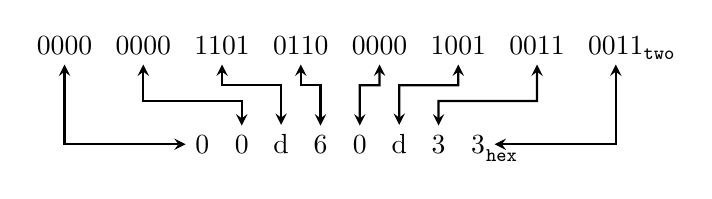
\begin{tikzpicture}[node distance=2cm]
        
        %32 bit instruction
        \node at (0,0) [text centered] (7) {0000};
        \node at (1,0) [text centered] (6) {0000};
        \node at (2,0) [text centered] (5) {1101};
        \node at (3,0) [text centered] (4) {0110};
        \node at (4,0) [text centered] (3) {0000};
        \node at (5,0) [text centered] (2) {1001};
        \node at (6,0) [text centered] (1) {0011};
        \node at (7,0) [text centered] (0) {0011};
        \node at (7.5,-0.1) [text centered] {$\; \texttt{\scriptsize two}$};
        
        
        
        %hex instrucion
        \node at (1.75,-1.25) [text centered] (h) {0};
        \node at (2.25  ,-1.25) [text centered] (g) {0};
        \node at (2.75,-1.25) [text centered] (f) {d};
        \node at (3.25  ,-1.25) [text centered] (e) {6};
        \node at (3.75,-1.25) [text centered] (d) {0};
        \node at (4.25  ,-1.25) [text centered] (c) {d};
        \node at (4.75,-1.25) [text centered] (b) {3};
        \node at (5.25  ,-1.25) [text centered] (a) {3};
        
        %Arrows
        \draw [arrow] (7) |- (h);
        \draw [arrow] (6) -- ++(0,-0.7) -- ++(1.25,0) -- (g);
        \draw [arrow] (5) -- ++(0,-0.5) -- ++(0.75,0) -- (f);
        \draw [arrow] (4) -- ++(0,-0.5) -- ++(0.25,0) -- (e);
        \draw [arrow] (3) -- ++(0,-0.5) -- ++(-0.25,0) -- (d);
        \draw [arrow] (2) -- ++(0,-0.5) -- ++(-0.75,0) -- (c);
        \draw [arrow] (1) -- ++(0,-0.7) -- ++(-1.25,0) -- (b);
        \draw [arrow] (0) |- (a);
        \node at (5.5,-1.40) [text centered] {$\; \texttt{\scriptsize hex}$};
    
    \end{tikzpicture}
\end{document}
